%%%%%%%%%%%%%%%%%%%%%%%%%%%%%%%%%%%%%%%%%
% Developer CV
% LaTeX Class
% Version 2.0 (21/05/2023)
%
% Authors:
% Will Fantom (willf@ntom.dev)
% Based on a template by Jan Küster (info@jankuester.com) and Jan Vorisek (jan@vorisek.me)
%
% License:
% The MIT License (see included LICENSE file)
%
%%%%%%%%%%%%%%%%%%%%%%%%%%%%%%%%%%%%%%%%%

%----------------------------------------------------------------
%	PACKAGES AND OTHER DOCUMENT CONFIGURATIONS
%----------------------------------------------------------------

\documentclass[9pt]{developercv} % Default font size, values from 8-12pt are recommended

%----------------------------------------------------------------

\begin{document}

%----------------------------------------------------------------
%	TITLE AND CONTACT INFORMATION
%----------------------------------------------------------------

\begin{minipage}[t]{0.38\textwidth} % 38% of the page width for name
	\vspace{-\baselineskip} % Required for vertically aligning minipages

	% If your name is very short, use just one of the lines below
	% If your name is very long, reduce the font size or make the minipage wider and reduce the others proportionately
	\colorbox{black}{{\HUGE\textcolor{white}{\textbf{\MakeUppercase{Paul}}}}}\hspace{0.35cm}\footnotesize{(he/him)} % First name

	\colorbox{black}{{\HUGE\textcolor{white}{\textbf{\MakeUppercase{Alcock}}}}} % Last name

	\vspace{6pt}

	{\huge Researcher, Tinkerer,\\ Developer, Nerd} % Career or current job title
\end{minipage}
\begin{minipage}[t]{0.22\textwidth} % 27.5% of the page width for the first row of icons
	\vspace{-\baselineskip} % Required for vertically aligning minipages

	% The first parameter is the FontAwesome icon name, the second is the box size and the third is the text
	% Other icons can be found by referring to fontawesome.pdf (supplied with the template) and using the word after \fa in the command for the icon you want
	\icon{MapMarker}{12}{buckshaw village, uk}\\
	\icon{Phone}{12}{+44 792 936 1133}\\
	\icon{At}{12}{\href{mailto:paul@alcock.dev}{paul@alcock.dev}}\\
\end{minipage}
\begin{minipage}[t]{0.22\textwidth} % 27.5% of the page width for the second row of icons
	\vspace{-\baselineskip} % Required for vertically aligning minipages
	\icon{Globe}{12}{\href{https://alcock.dev}{alcock.dev}}\\
	\icon{Github}{12}{\href{https://github.com/guilvareux}{@guilvareux}}\\
	\icon{Linkedin}{12}{\href{https://linkedin.com/in/paulalcock}{@paulalcock}}\\
\end{minipage}
\begin{minipage}[t]{0.18\textwidth} % 18% of the page width for pic
	\vspace{-\baselineskip} % Required for vertically aligning minipages
	\hfill
	{%
		\setlength{\fboxsep}{0pt}%
		\setlength{\fboxrule}{5pt}%
		\fbox{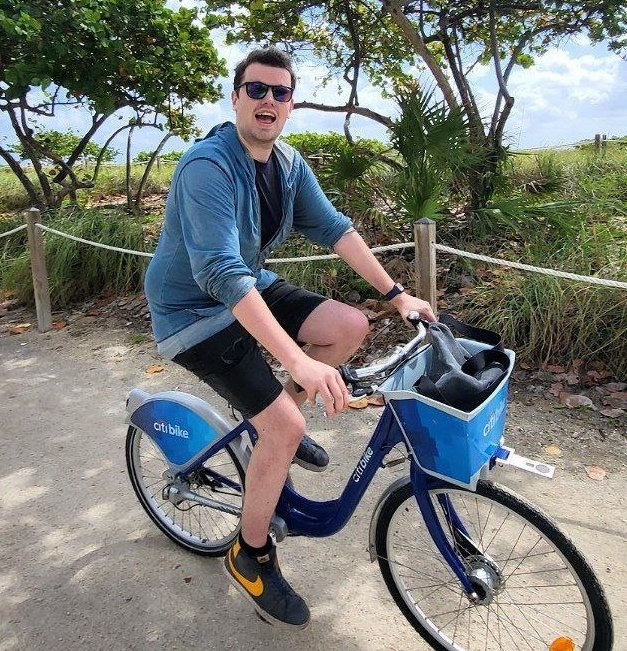
\includegraphics[width=0.8\linewidth]{assets/profile.jpg}}%
	}%
\end{minipage}

\vspace{0.15cm}

%----------------------------------------------------------------
%	INTRODUCTION, SKILLS AND TECHNOLOGIES
%----------------------------------------------------------------

\cvsect{Who Am I?}

\begin{minipage}[t]{0.35\textwidth} % 40% of the page width for the introduction text
	\vspace{-\baselineskip} % Required for vertically aligning minipages

	I am a network researcher and PhD student with a focus on network and cloud
	infrastructures. The opportunities I have had to work alongside large tech
	companies in my research as they adopt modern software deployment workflows
	has allowed me to design and develop novel tools for network management and
	orchestration. I typically spend my weekends on homelab projects and
	cooking.\\
\end{minipage}
\hfill % Whitespace between
\begin{minipage}[t]{0.31\textwidth} % 50% of the page for the skills bar chart
	\vspace{-\baselineskip} % Required for vertically aligning minipages
	\begin{barchart}{4.1}
		\baritem{Python}{82}
		\baritem{Rust}{100}
		\baritem{Golang}{68}
		\baritem{Prolog}{60}
		\baritem{LaTeX}{50}
		\baritem{Git}{80}
	\end{barchart}
\end{minipage}
\hfill % Whitespace between
\begin{minipage}[t]{0.29\textwidth} % 50% of the page for the skills bar chart
	\vspace{-\baselineskip}\vspace{-\baselineskip} % Required for vertically aligning minipages
	\cvsect{Tools}\\
	\mbox{\cvtag{Docker}\cvtag{LibVirt}\cvtag{Openstack}}
	\mbox{\cvtag{Kubernetes}\cvtag{Obsidian}\cvtag{Linux}}
	\mbox{\cvtag{GitHub Actions}\cvtag{QGIS}\cvtag{Nix}}
	\mbox{\cvtag{Grafana}\cvtag{Neovim}\cvtag{Ansible}}
	\mbox{\cvtag{Prometheus}}
\end{minipage}

%----------------------------------------------------------------
%	EXPERIENCE
%----------------------------------------------------------------

\vspace{-1em}
\cvsect{Experience}

\begin{entrylist}
	\entry
	{2024 -- Present}
	{Research Associate: TUDOR}
	{Lancaster University}
	{Working in a multi-Univeristy partnership to deliver a smart,
	intent-based network infrastructure, enabling autonomic network management,
	guided by abstract, high-level goals.\\
		\texttt{Rust}\slashsep\texttt{Prolog}\slashsep\texttt{Kubernetes}\slashsep\texttt{Openstack}\slashsep\texttt{Nomad}\slashsep\texttt{Linux}}
	\entry
	{2023 -- 2023}
	{Research Associate: Future Places Centre}
	{Lancaster University}
	{Analyzing a socio-economic dataset for a local food charity, aiming to
	explore and understand local demographic information and communicate
	findings to aid engagement with local community.\\
		\texttt{Python}\slashsep\texttt{QGIS}\slashsep\texttt{Linux}}
	\entry
	{2021 -- 2023\\\footnotesize{part time}}
	{Graduate Teaching Assistant}
	{Lancaster University}
	{Assisted the delivery of Networking, Advanced Networking and Distrbuted
	Systems courses at Lancaster University.\\
		\texttt{Python}\slashsep\texttt{Java}\slashsep\texttt{Mininet}\slashsep\texttt{Openflow}\slashsep\texttt{Docker}\slashsep\texttt{JGroups}}
	%\entry
	%{2020 -- 2022\\\footnotesize{part time}}
	%{Research Associate: NG-CDI}
	%{Lancaster University}
	%{Worked alongside BT and other academic partners to investigate how cloud
	%	practices (primarily DevOps) could be utilized in network infrastructure as
	%	they transition from hardware-based deployments to software.\\
	%	\texttt{Go}\slashsep\texttt{C}\slashsep\texttt{GitHub Actions}\slashsep\texttt{Unikraft}\slashsep\texttt{Prometheus}\slashsep\texttt{Grafana}\slashsep\texttt{Træfik}}
\end{entrylist}

%----------------------------------------------------------------
%	EDUCATION
%----------------------------------------------------------------

\vspace{-1em}
\cvsect{Education}

\begin{entrylist}
	\entry
	{2021 -- present\\\footnotesize{ending approx. 2025}}
	{PhD -- Computer Science}
	{Lancaster University}
	{Working to design and implement an extensible intent handler using semantic
	web technologies and logic programming, to enable autonomic network
	management for 5G network infrastructure.
	\\\texttt{Intent-based
	Networking}\slashsep\texttt{Orchestration}\slashsep\texttt{Cloud}\slashsep\texttt{CI/CD}\slashsep\texttt{NetDevOps}}
	\entry
	{2016 -- 2020}
	{BSc (Hons) Computer Science \textit{(2:1)}}
	{Lancaster University}
	{Thesis included the creation and evaluation of a virtual reality
	experience, for educating students about binary tree traversals
	\\\texttt{Artificial Intelligence}\slashsep\texttt{Adv.
			Programming}\slashsep\texttt{Adv. Networking}\slashsep\texttt{Distributed Systems}\slashsep\texttt{...}}
\end{entrylist}

%----------------------------------------------------------------
%	PUBLICATIONS
%----------------------------------------------------------------

\vspace{-1em}
\cvsect{Publications}

\begin{entrylist}
	\pubentry
	{2024}
	{[1st Author]}
	{Oz: Towards an Extensible Intent Handler Architecture with Semantic
	Reasoning}
	{IEEE/Netsoft}
	\pubentry
	{2022}
	{[1st Author]}
	{Improving Intent Correctness with Automated Testing}
	{IEEE/Netsoft}
	\pubentry
	{2022}
	{}
	{A NEAT way to test-driven network management}
	{IEEE/IFIP NOMS}
\end{entrylist}

%----------------------------------------------------------------
% ADDITIONAL INFORMATION
%----------------------------------------------------------------

\begin{minipage}[t]{0.35\textwidth}
	\vspace{-\baselineskip} % Required for vertically aligning minipages
	\cvsect{Hobbies}\\
	\cvtag{Homelab}\cvtag{3D Printing}\cvtag{Cooking}
	\cvtag{Motorcycles}\cvtag{Coffee}\cvtag{Music}
	\divider\\
	\begin{minipage}[t]{0.25\textwidth}
		\vspace{-\baselineskip} % Required for vertically aligning minipages
		
\includegraphics[width=1\linewidth]{assets/websiteqr.png}
	\end{minipage}
	\hfill
	\begin{minipage}[t]{0.75\textwidth}
		\vspace{-\baselineskip} % Required for vertically aligning minipages
		Scan this QR Code to make sure you are seeing the latest version of my CV.\\
		Compiled on \textit{\today}\\
	\end{minipage}
\end{minipage}
\hfill
\begin{minipage}[t]{0.6\textwidth}
	\vspace{-\baselineskip} % Required for vertically aligning minipages
	\cvsect{Project: Oz}\\
	Lead developer on a first of a kind intent handler design, aiming to
	automate aspects of network management through high-level, abstract
	requirements. Oz leverages semantic web technologies and logic programming
	to interpret abstract goals as policies, enabling new network configurations
	to be generated as constraint satisfaction problems. Once a network
	configuration is created, Oz additionally has the ability to interface with
	orchestrators to support self: configuration, healing, optimisation and
	protection of network services. All development work was achieved with
	Prolog and Rust programming languages combined with Nix to manage
	development environments and CI/CD. This work is currently being explored as
	part of the TUDOR project, forming the basis of one of the major
	deliverables for 5G network management.
\end{minipage}

%----------------------------------------------------------------

\end{document}
